\documentclass{article}
\usepackage{xcolor}
\usepackage{hyperref}
\usepackage[utf8]{inputenc}
\usepackage{graphicx}
\graphicspath{ {./images/} }
\title{Sentiment Analysis in Julia}
\author{Andrew Lee \\ \href{mailto:andrewlee733@u.boisestate.edu}{\color{blue}{andrewlee733@u.boisestate.edu}}
    \and Josh Coward \\ \href{mailto:joshcoward@u.boisestate.edu}{\color{blue}{joshcoward@u.boisestate.edu}} }

\date{October 14, 2020}

\begin{document}

\maketitle

\begin{abstract}
Through the use of a high level, high performance, general purpose programming language called Julia, we are proposing to develop a sentiment analysis machine learning model to detect whether or not a statement/sentence contains a positive, negative, or neutral message. We then want to develop a small GUI to present our findings, and also allow users to test out their own sentences on our model. If there's time remaining we will re implement our model using Julia's built in multi-threading library to determine if there's a substantial change in efficiency between training the models in our single and multi-threaded implementations.
\end{abstract}

\begin{figure}[h]
\caption{Julia logo, \protect\cite{Julia2020}}
\begin{center}

\includegraphics{juliaLogo}
\end{center}
\end{figure}

\section{Introduction}
Our chosen language, Julia, is a high level, high performance, general purpose programming language. Since Julia is designed for computational science, our motivation behind this project comes from wanting to explore this aspect by creating a machine learning model capable of making accurate predictions and presenting that information in a GUI. If time permits it, we also plan on utilizing Julia's Multi-threaded capabilities to see what speedups we get compared to our single threaded version, as well as compare our model training time to an implementation using the most popular machine learning programming language, Python. We also intend to create additional machine learning models over different data sets to show off how Julia can be used for fast prototyping, but since we do not have a large amount of experience in machine learning this also depends on the speed of our progress.

\section{Project Description}
The plan for the project is to explore the Julia programming language and its data science libraries in order to build a sentiment analysis model using the Sentiment140 data set. The goal is to get a prediction accuracy of 90\% or better on the test data set and then we want to take advantage of Julia's data visualization libraries in order to both explore the data set itself but to also present our findings in a GUI for the user to see, because as stated on Julia's website "Data Visualization has a complicated history. Plotting software makes trade-offs between features and simplicity, speed and beauty, and a static and dynamic interface."\cite{Julia2020-2} By using Julia for this task we hope to eliminate these trade offs.If time allows it, we would also like to break the data set up into subsections where we can then process each subsection at the same time using Julia's built in multi-threaded libraries in order to speed up the training time of the model. We then want to compare the speed of training our model using our original single threaded approach vs the multi-threaded approach in order to see if there is a clear difference between the two. This would ultimately tell us whether or not the Julia programming language and its faster efficiency make it worth being used over python in the data science/machine learning industry.
 
\section{Evaluation}

\subsection{Model}
To evaluate the success of our machine learning model, we will verify that the model has an accuracy of 90\% or better at determining the category of a post on the Sentiment140 data set. The data set contains over one million Twitter posts that have been categorized into three groups: positive, negative, and neutral. If a post is marked as positive, it means that the text has an overall positive sentiment, such as "Today was a good day :)". Likewise, if a post is marked as negative the overall sentiment is negative, and for neutral the sentiment is either unclear or indifferent. Since the data set is explicitly marked with the sentiment of each post, it will be simple to test the accuracy of our model once it has been trained. Additionally, we want our code to be straightforward and easy to read, since Julia is marketed as a high level language that excels at fast prototyping.

\subsection{Graphical User Interface}
Our graphical user interface will consist of at least three main components. The first will plot the loss function over the time of training the model, and shows the expected loss value in real time as the model is being trained. The second will be used after the model has finished training, and generates a list of words that show up often in either positive, negative, or neutral posts in order to give some idea between words and their inherent sentiment. The third component will accepts text input from the user and outputs whether their input is either positive, negative, or neutral, according to the model. We are evaluating this component based off of whether these three features are present in a simple, intuitive interface and contain accurate data that reflects our model. We may add more components in addition to these, but these three are considered necessary.
\begin{figure}[h]
\caption{Julia's built-in data visualization library, Plots.jl, \protect\cite{Julia2020-2}}
\begin{center}
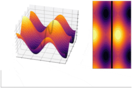
\includegraphics{waves}
\end{center}
\end{figure}

\subsection{Multi-threading}
To evaluate the our implementation of multi-threading, we will compare the model training time between our single-threaded and multi-threaded versions of our project. Both models will be considered done once they have reached 90\% accuracy. If there is a speedup of at least 50\% in the multi-threaded version, we will conclude that multi-threading was worth the effort for our project. We will also create a set of tests to try to ensure there are no race conditions in our multi-threaded implementation, which will work as a pass/fail to determine whether the multi-threaded implementation is valid for real world use. Since race conditions are hard to test due to the inherent non-determinism of multi-threading, we cannot guarantee that all possible race conditions will be accounted for, only that we will attempt to catch them all. Lastly, we will rewrite our multi-threaded implementation in Python, and again train two models on the multi-threaded implementations in Julia and Python to 90\% accuracy. If the Julia model has at least a 50\% speedup over the Python model in training, we will conclude that there is a substantial advantage to using Julia over Python in a machine learning context.

\subsection{Additional Models}
Since these models are not the main focus of our project, less effort will be made to ensure the effectiveness of the models. If the model's have a success rate of at least 80\%, we will consider them good enough. In the case where there is no concrete way to determine accuracy in a model, we will judge the model based on whether it provides us useful or interesting information about whatever data set it is using. We will also evaluate how easy it was to implement these models using Julia, and judge Julia's claim of fast prototyping based on how much time it takes to create these additional models.

\section{Management}
Our means of communicating and collaborating for this project is through Slack and a shared GitHub repository. While both of us plan on working on each of the milestones equally, we have decided that one of us is going to focus slightly more energy on building the machine learning model and the other person is going to be focusing slightly more on the GUI and if time allows more so on the multi-threading as well. The first week will be spent learning Julia through documentation and test programs, and the remaining five will be used working on the main project.

\begin{table*}[ht]
\centering
\begin{tabular}{c|c}
\hline
\textbf{Week} & \textbf{Main Focus}\\
\hline
\textbf{1} & Learn Julia \\
\textbf{2} & Build ML Model \\
\textbf{3} & Build ML Model \\
\textbf{4} & Build GUI \\
\textbf{5} & Add Multi-threading \\
\textbf{6} & Create Additional Models \\
\end{tabular}
\end{table*}

\bibliographystyle{plainnat}
\bibliography{refs}

\end{document}
